\documentclass[11pt,a4paper]{article}
\usepackage[a4paper,margin=24mm,headheight=14pt]{geometry}
\usepackage{fontspec}
\setmainfont{TeX Gyre Pagella}
\setsansfont{TeX Gyre Heros}
\setmonofont{DejaVu Sans Mono}[Scale=0.85]
\newfontfamily\rupeefont{DejaVu Sans}
\newcommand{\rupee}{{\rupeefont ₹}}
\usepackage{microtype}
\usepackage{amsmath,amssymb}
\usepackage{graphicx}
\usepackage{booktabs,tabularx,multirow}
\usepackage{xcolor}
\usepackage{tikz}
\usetikzlibrary{positioning,arrows.meta,calc,fit}
\usepackage[most]{tcolorbox}
\usepackage{enumitem}
\usepackage{titlesec}
\usepackage{fancyhdr}
\usepackage{caption}
\usepackage[hidelinks]{hyperref}
\usepackage{float}
\setlength{\emergencystretch}{2em}
\setcounter{tocdepth}{2}
\setcounter{secnumdepth}{2}
\usepackage{array}
\newcolumntype{L}{>{\raggedright\arraybackslash}X}

\definecolor{ink}{HTML}{1D2327}
\definecolor{muted}{HTML}{5B666C}
\definecolor{accent}{HTML}{1F6F6B}
\definecolor{lever}{HTML}{2A78D6}
\definecolor{package}{HTML}{4A3AA7}
\definecolor{suppression}{HTML}{EB6834}
\definecolor{paper}{HTML}{F4F6F4}

\titleformat{\section}{\sffamily\Large\bfseries\color{ink}}{\thesection}{0.7em}{}
\titleformat{\subsection}{\sffamily\large\bfseries\color{ink}}{\thesubsection}{0.6em}{}
\titleformat{\subsubsection}{\sffamily\normalsize\bfseries\color{accent}}{}{0em}{}
\titlespacing*{\subsubsection}{0pt}{1.1ex}{0.4ex}
\captionsetup{font={small,sf},labelfont=bf}
\setlist{itemsep=2pt,topsep=4pt}
\pagestyle{fancy}
\fancyhf{}
\fancyhead[L]{\sffamily\footnotesize\color{muted}Designing Reservation Reform Without Mass Unrest}
\fancyhead[R]{\sffamily\footnotesize\color{muted}Research report}
\fancyfoot[C]{\sffamily\footnotesize\thepage}
\renewcommand{\headrulewidth}{0pt}

\newtcolorbox{plainwords}{colback=paper,colframe=paper,boxrule=0pt,arc=2pt,left=8pt,right=8pt,top=5pt,bottom=5pt,
  fontupper=\small,before upper={\textsf{\textbf{\color{accent}In plain words.}}\ }}
\newtcolorbox{keyresult}[1][]{colback=white,colframe=accent,boxrule=0.6pt,arc=2pt,left=8pt,right=8pt,top=6pt,bottom=6pt,
  fonttitle=\sffamily\bfseries\small,coltitle=white,colbacktitle=accent,title=#1}

\newcommand{\outcomeline}[6]{%
  \begin{tabular}{@{}llll@{}}
  \sffamily\small\color{muted}Peak day (grounded) & \sffamily\small\color{muted}Change & \sffamily\small\color{muted}Ever protested & \sffamily\small\color{muted}Deaths\\
  \textbf{#1} \small(#2) & \textbf{#3} & #4 & #5\\
  \end{tabular}\par\smallskip
  {\small\color{muted}Stylized specification: #6}\par}

\newcommand{\PeakCentralBaseline}{46.1~lakh}
\newcommand{\PeakRangeCentralBaseline}{14.9--118.9}
\newcommand{\PeakChangeCentralBaseline}{0\%}
\newcommand{\CumulativeCentralBaseline}{1.29~crore}
\newcommand{\CumulativeChangeCentralBaseline}{0\%}
\newcommand{\DeathsCentralBaseline}{18.5}
\newcommand{\DeathRatioCentralBaseline}{1.0}
\newcommand{\PeakCentralGrandfathering}{15.6~lakh}
\newcommand{\PeakRangeCentralGrandfathering}{6.6--41.5}
\newcommand{\PeakChangeCentralGrandfathering}{$-$66\%}
\newcommand{\CumulativeCentralGrandfathering}{0.50~crore}
\newcommand{\CumulativeChangeCentralGrandfathering}{$-$61\%}
\newcommand{\DeathsCentralGrandfathering}{5.5}
\newcommand{\DeathRatioCentralGrandfathering}{0.3}
\newcommand{\PeakCentralSeatExpansion}{24.1~lakh}
\newcommand{\PeakRangeCentralSeatExpansion}{9.8--65.8}
\newcommand{\PeakChangeCentralSeatExpansion}{$-$48\%}
\newcommand{\CumulativeCentralSeatExpansion}{0.74~crore}
\newcommand{\CumulativeChangeCentralSeatExpansion}{$-$43\%}
\newcommand{\DeathsCentralSeatExpansion}{11}
\newcommand{\DeathRatioCentralSeatExpansion}{0.6}
\newcommand{\PeakCentralHybridCasteSubquotas}{2.9~lakh}
\newcommand{\PeakRangeCentralHybridCasteSubquotas}{1.7--4.3}
\newcommand{\PeakChangeCentralHybridCasteSubquotas}{$-$94\%}
\newcommand{\CumulativeCentralHybridCasteSubquotas}{0.10~crore}
\newcommand{\CumulativeChangeCentralHybridCasteSubquotas}{$-$92\%}
\newcommand{\DeathsCentralHybridCasteSubquotas}{1}
\newcommand{\DeathRatioCentralHybridCasteSubquotas}{0.1}
\newcommand{\PeakCentralSubClassification}{26.9~lakh}
\newcommand{\PeakRangeCentralSubClassification}{11.6--71.4}
\newcommand{\PeakChangeCentralSubClassification}{$-$42\%}
\newcommand{\CumulativeCentralSubClassification}{0.83~crore}
\newcommand{\CumulativeChangeCentralSubClassification}{$-$36\%}
\newcommand{\DeathsCentralSubClassification}{13.5}
\newcommand{\DeathRatioCentralSubClassification}{0.7}
\newcommand{\PeakCentralConsensusCommission}{8.3~lakh}
\newcommand{\PeakRangeCentralConsensusCommission}{4.1--24.2}
\newcommand{\PeakChangeCentralConsensusCommission}{$-$82\%}
\newcommand{\CumulativeCentralConsensusCommission}{0.41~crore}
\newcommand{\CumulativeChangeCentralConsensusCommission}{$-$68\%}
\newcommand{\DeathsCentralConsensusCommission}{4.5}
\newcommand{\DeathRatioCentralConsensusCommission}{0.2}
\newcommand{\PeakCentralCompensation}{34.9~lakh}
\newcommand{\PeakRangeCentralCompensation}{13.1--93.9}
\newcommand{\PeakChangeCentralCompensation}{$-$24\%}
\newcommand{\CumulativeCentralCompensation}{1.08~crore}
\newcommand{\CumulativeChangeCentralCompensation}{$-$16\%}
\newcommand{\DeathsCentralCompensation}{16.5}
\newcommand{\DeathRatioCentralCompensation}{0.9}
\newcommand{\PeakCentralCredibleGuarantees}{18.2~lakh}
\newcommand{\PeakRangeCentralCredibleGuarantees}{9.6--55.2}
\newcommand{\PeakChangeCentralCredibleGuarantees}{$-$61\%}
\newcommand{\CumulativeCentralCredibleGuarantees}{0.68~crore}
\newcommand{\CumulativeChangeCentralCredibleGuarantees}{$-$47\%}
\newcommand{\DeathsCentralCredibleGuarantees}{7.5}
\newcommand{\DeathRatioCentralCredibleGuarantees}{0.4}
\newcommand{\PeakCentralInternetShutdown}{42.8~lakh}
\newcommand{\PeakRangeCentralInternetShutdown}{17.2--73.7}
\newcommand{\PeakChangeCentralInternetShutdown}{$-$7\%}
\newcommand{\CumulativeCentralInternetShutdown}{1.41~crore}
\newcommand{\CumulativeChangeCentralInternetShutdown}{+9\%}
\newcommand{\DeathsCentralInternetShutdown}{54.5}
\newcommand{\DeathRatioCentralInternetShutdown}{2.9}
\newcommand{\PeakCentralHeavyPolicing}{32.9~lakh}
\newcommand{\PeakRangeCentralHeavyPolicing}{17.4--73.3}
\newcommand{\PeakChangeCentralHeavyPolicing}{$-$29\%}
\newcommand{\CumulativeCentralHeavyPolicing}{1.61~crore}
\newcommand{\CumulativeChangeCentralHeavyPolicing}{+25\%}
\newcommand{\DeathsCentralHeavyPolicing}{79.5}
\newcommand{\DeathRatioCentralHeavyPolicing}{4.3}
\newcommand{\PeakCentralManagedTransition}{2.2~lakh}
\newcommand{\PeakRangeCentralManagedTransition}{1.4--3.4}
\newcommand{\PeakChangeCentralManagedTransition}{$-$95\%}
\newcommand{\CumulativeCentralManagedTransition}{0.12~crore}
\newcommand{\CumulativeChangeCentralManagedTransition}{$-$91\%}
\newcommand{\DeathsCentralManagedTransition}{1}
\newcommand{\DeathRatioCentralManagedTransition}{0.1}
\newcommand{\PeakCentralHybridPackage}{0.6~lakh}
\newcommand{\PeakRangeCentralHybridPackage}{0.4--0.9}
\newcommand{\PeakChangeCentralHybridPackage}{$-$99\%}
\newcommand{\CumulativeCentralHybridPackage}{0.04~crore}
\newcommand{\CumulativeChangeCentralHybridPackage}{$-$97\%}
\newcommand{\DeathsCentralHybridPackage}{0}
\newcommand{\DeathRatioCentralHybridPackage}{0.0}
\newcommand{\PeakCentralSymbolicOnlyValidation}{13.3~lakh}
\newcommand{\PeakRangeCentralSymbolicOnlyValidation}{6.0--37.6}
\newcommand{\PeakChangeCentralSymbolicOnlyValidation}{$-$71\%}
\newcommand{\CumulativeCentralSymbolicOnlyValidation}{0.47~crore}
\newcommand{\CumulativeChangeCentralSymbolicOnlyValidation}{$-$64\%}
\newcommand{\DeathsCentralSymbolicOnlyValidation}{5.5}
\newcommand{\DeathRatioCentralSymbolicOnlyValidation}{0.3}
\newcommand{\PeakHighBaseline}{2.09~crore}
\newcommand{\PeakRangeHighBaseline}{92.6--388.4}
\newcommand{\PeakChangeHighBaseline}{0\%}
\newcommand{\CumulativeHighBaseline}{4.14~crore}
\newcommand{\CumulativeChangeHighBaseline}{0\%}
\newcommand{\DeathsHighBaseline}{79}
\newcommand{\DeathRatioHighBaseline}{1.0}
\newcommand{\PeakHighGrandfathering}{74.2~lakh}
\newcommand{\PeakRangeHighGrandfathering}{20.0--160.7}
\newcommand{\PeakChangeHighGrandfathering}{$-$65\%}
\newcommand{\CumulativeHighGrandfathering}{1.98~crore}
\newcommand{\CumulativeChangeHighGrandfathering}{$-$52\%}
\newcommand{\DeathsHighGrandfathering}{30.5}
\newcommand{\DeathRatioHighGrandfathering}{0.4}
\newcommand{\PeakHighSeatExpansion}{1.17~crore}
\newcommand{\PeakRangeHighSeatExpansion}{35.5--258.0}
\newcommand{\PeakChangeHighSeatExpansion}{$-$44\%}
\newcommand{\CumulativeHighSeatExpansion}{2.50~crore}
\newcommand{\CumulativeChangeHighSeatExpansion}{$-$40\%}
\newcommand{\DeathsHighSeatExpansion}{45}
\newcommand{\DeathRatioHighSeatExpansion}{0.6}
\newcommand{\PeakHighHybridCasteSubquotas}{7.7~lakh}
\newcommand{\PeakRangeHighHybridCasteSubquotas}{5.1--12.5}
\newcommand{\PeakChangeHighHybridCasteSubquotas}{$-$96\%}
\newcommand{\CumulativeHighHybridCasteSubquotas}{0.29~crore}
\newcommand{\CumulativeChangeHighHybridCasteSubquotas}{$-$93\%}
\newcommand{\DeathsHighHybridCasteSubquotas}{3}
\newcommand{\DeathRatioHighHybridCasteSubquotas}{0.0}
\newcommand{\PeakHighSubClassification}{1.06~crore}
\newcommand{\PeakRangeHighSubClassification}{40.0--225.0}
\newcommand{\PeakChangeHighSubClassification}{$-$49\%}
\newcommand{\CumulativeHighSubClassification}{2.54~crore}
\newcommand{\CumulativeChangeHighSubClassification}{$-$39\%}
\newcommand{\DeathsHighSubClassification}{46.5}
\newcommand{\DeathRatioHighSubClassification}{0.6}
\newcommand{\PeakHighConsensusCommission}{42.2~lakh}
\newcommand{\PeakRangeHighConsensusCommission}{13.5--106.7}
\newcommand{\PeakChangeHighConsensusCommission}{$-$80\%}
\newcommand{\CumulativeHighConsensusCommission}{1.55~crore}
\newcommand{\CumulativeChangeHighConsensusCommission}{$-$63\%}
\newcommand{\DeathsHighConsensusCommission}{26.5}
\newcommand{\DeathRatioHighConsensusCommission}{0.3}
\newcommand{\PeakHighCompensation}{1.67~crore}
\newcommand{\PeakRangeHighCompensation}{49.3--327.2}
\newcommand{\PeakChangeHighCompensation}{$-$20\%}
\newcommand{\CumulativeHighCompensation}{3.80~crore}
\newcommand{\CumulativeChangeHighCompensation}{$-$8\%}
\newcommand{\DeathsHighCompensation}{65}
\newcommand{\DeathRatioHighCompensation}{0.8}
\newcommand{\PeakHighCredibleGuarantees}{1.11~crore}
\newcommand{\PeakRangeHighCredibleGuarantees}{34.9--247.2}
\newcommand{\PeakChangeHighCredibleGuarantees}{$-$47\%}
\newcommand{\CumulativeHighCredibleGuarantees}{2.52~crore}
\newcommand{\CumulativeChangeHighCredibleGuarantees}{$-$39\%}
\newcommand{\DeathsHighCredibleGuarantees}{43}
\newcommand{\DeathRatioHighCredibleGuarantees}{0.5}
\newcommand{\PeakHighInternetShutdown}{1.11~crore}
\newcommand{\PeakRangeHighInternetShutdown}{55.9--184.4}
\newcommand{\PeakChangeHighInternetShutdown}{$-$47\%}
\newcommand{\CumulativeHighInternetShutdown}{3.43~crore}
\newcommand{\CumulativeChangeHighInternetShutdown}{$-$17\%}
\newcommand{\DeathsHighInternetShutdown}{152.5}
\newcommand{\DeathRatioHighInternetShutdown}{1.9}
\newcommand{\PeakHighHeavyPolicing}{1.24~crore}
\newcommand{\PeakRangeHighHeavyPolicing}{52.4--245.6}
\newcommand{\PeakChangeHighHeavyPolicing}{$-$41\%}
\newcommand{\CumulativeHighHeavyPolicing}{4.20~crore}
\newcommand{\CumulativeChangeHighHeavyPolicing}{+1\%}
\newcommand{\DeathsHighHeavyPolicing}{254.5}
\newcommand{\DeathRatioHighHeavyPolicing}{3.2}
\newcommand{\PeakHighManagedTransition}{6.4~lakh}
\newcommand{\PeakRangeHighManagedTransition}{3.6--10.0}
\newcommand{\PeakChangeHighManagedTransition}{$-$97\%}
\newcommand{\CumulativeHighManagedTransition}{0.36~crore}
\newcommand{\CumulativeChangeHighManagedTransition}{$-$91\%}
\newcommand{\DeathsHighManagedTransition}{4}
\newcommand{\DeathRatioHighManagedTransition}{0.1}
\newcommand{\PeakHighHybridPackage}{1.9~lakh}
\newcommand{\PeakRangeHighHybridPackage}{1.3--2.9}
\newcommand{\PeakChangeHighHybridPackage}{$-$99\%}
\newcommand{\CumulativeHighHybridPackage}{0.12~crore}
\newcommand{\CumulativeChangeHighHybridPackage}{$-$97\%}
\newcommand{\DeathsHighHybridPackage}{1}
\newcommand{\DeathRatioHighHybridPackage}{0.0}
\newcommand{\PeakHighSymbolicOnlyValidation}{66.1~lakh}
\newcommand{\PeakRangeHighSymbolicOnlyValidation}{18.0--152.5}
\newcommand{\PeakChangeHighSymbolicOnlyValidation}{$-$68\%}
\newcommand{\CumulativeHighSymbolicOnlyValidation}{1.84~crore}
\newcommand{\CumulativeChangeHighSymbolicOnlyValidation}{$-$56\%}
\newcommand{\DeathsHighSymbolicOnlyValidation}{27}
\newcommand{\DeathRatioHighSymbolicOnlyValidation}{0.3}
\newcommand{\HybridRetainedForty}{2.7~lakh}
\newcommand{\HybridRetainedSixty}{4.6~lakh}
\newcommand{\HybridRetainedEighty}{9.2~lakh}
\newcommand{\ManagedTransitionFull}{2.2~lakh}
\newcommand{\ManagedTransitionWithoutGrandfatherCurrentCohortsWithTenYearGlide}{2.9~lakh}
\newcommand{\ManagedTransitionWithoutExpandSeatsSoNoGroupLoses}{2.6~lakh}
\newcommand{\ManagedTransitionWithoutBuildConsensusThroughDataFirstCommission}{6.6~lakh}
\newcommand{\ManagedTransitionWithoutCompensateAboveLineLosers}{2.4~lakh}
\newcommand{\ManagedTransitionWithoutGuaranteeUntouchedProtections}{3.6~lakh}

\newcommand{\HistOnePeak}{98.0~crore}
\newcommand{\HistOneBandhSC}{30.6\%}
\newcommand{\HistOneBandhST}{17.3\%}
\newcommand{\HistOneBandhOBC}{1.6\%}
\newcommand{\HistOneBandhGeneral}{0.0\%}
\newcommand{\HistFinalBandhSC}{0.70\%}
\newcommand{\HistFinalBandhST}{0.26\%}
\newcommand{\HistFinalBandhOBC}{0.05\%}
\newcommand{\HistFinalBandhGeneral}{0.00\%}
\newcommand{\HistTwoBaseline}{30.5~lakh}
\newcommand{\HistTwoBaselineRange}{7.1--457.6}
\newcommand{\HistTwoSymbolicOnly}{10{,}000}
\newcommand{\HistTwoSymbolicShare}{0.3\%}
\newcommand{\HistTwoChangeGrandfathering}{$-$99\%}
\newcommand{\HistTwoChangeHybrid}{$-$92\%}
\newcommand{\HistTwoChangeConsensus}{$-$87\%}
\newcommand{\HistTwoChangeCompensation}{$-$91\%}
\newcommand{\HistTwoChangeManaged}{$-$100\%}
\newcommand{\HistTwoFallFactor}{3.1}
\newcommand{\HistTwoPeakAtFourNine}{2.6~crore}
\newcommand{\HistTwoPeakAtFive}{86.6~lakh}
\newcommand{\HistFinalFallFactor}{2.3}
\newcommand{\FinalSymbolicShare}{29\%}
\newcommand{\SensReferencePeak}{42.7~lakh}
\newcommand{\SensPerturbationCount}{24}
\newcommand{\SensRankCorrMin}{0.93}
\newcommand{\SensRankCorrMedian}{1.00}
\newcommand{\SensHybridStrongestCount}{24}
\newcommand{\SensCompensationWeakestCount}{21}
\newcommand{\SensWidestParameter}{threshold spread}
\newcommand{\SensWidestLow}{5.8~lakh}
\newcommand{\SensWidestHigh}{2.2~crore}
\newcommand{\SensWeakestSummary}{L6 in 21, L4 in 3}
\newcommand{\ParamLossAversion}{2.25}
\newcommand{\ParamMeanThreshold}{6.6}

\newcommand{\EligibilityLose}{6.8\%}
\newcommand{\EligibilityGain}{3.1\%}
\newcommand{\EligibilityLoseRange}{5.2\%--8.3\%}
\newcommand{\EligibilityGainRange}{1.0\%--5.1\%}
\newcommand{\EligibilityOriginal}{2.9\%}
\newcommand{\EligibilitySCSTAbove}{2.9\%}
\newcommand{\AllocYears}{2021--2025}
\newcommand{\AllocDraws}{300}
\newcommand{\AllocDrawsKept}{1{,}500}
\newcommand{\AllocMaxDecileError}{3.5}
\newcommand{\AllocGapEWSOBC}{0.012}
\newcommand{\AllocGapSCSTOthers}{0.03}
\newcommand{\AllocGapSCSTWorstYear}{2023}
\newcommand{\AllocGapSCSTWorst}{0.126}
\newcommand{\AllocMaxAllotmentGap}{406}
\newcommand{\AllocMaxAllotmentGapOpenFirst}{2{,}386}
\newcommand{\AllocChangeSCAbove}{$-$96\%}
\newcommand{\AllocRelSCAbove}{1.00}
\newcommand{\AllocChangeSCBelow}{$-$72\%}
\newcommand{\AllocRelSCBelow}{0.66}
\newcommand{\AllocChangeSTAbove}{$-$98\%}
\newcommand{\AllocRelSTAbove}{1.09}
\newcommand{\AllocChangeSTBelow}{$-$85\%}
\newcommand{\AllocRelSTBelow}{0.84}
\newcommand{\AllocChangeOBCAbove}{$-$87\%}
\newcommand{\AllocRelOBCAbove}{0.74}
\newcommand{\AllocChangeOBCBelow}{+23\%}
\newcommand{\AllocRelOBCBelow}{$-$0.16}
\newcommand{\AllocChangeEWS}{+71\%}
\newcommand{\AllocRelEWS}{$-$0.45}
\newcommand{\AllocChangeGENBelow}{+158\%}
\newcommand{\AllocRelGENBelow}{$-$2.61}
\newcommand{\AllocChangeGENAbove}{$-$10\%}
\newcommand{\AllocRelGENAbove}{0.18}
\newcommand{\AllocExpandedSCAbove}{$-$95\%}
\newcommand{\AllocExpandedSCBelow}{$-$63\%}
\newcommand{\AllocExpandedSTAbove}{$-$97\%}
\newcommand{\AllocExpandedSTBelow}{$-$79\%}
\newcommand{\AllocExpandedOBCAbove}{$-$83\%}
\newcommand{\AllocExpandedOBCBelow}{+57\%}
\newcommand{\AllocExpandedEWS}{+116\%}
\newcommand{\AllocExpandedGENBelow}{+211\%}
\newcommand{\AllocExpandedGENAbove}{+11\%}
\newcommand{\AllocFilterSCAbove}{$-$97\%}
\newcommand{\AllocFilterSCBelow}{+32\%}
\newcommand{\AllocFilterSTAbove}{$-$98\%}
\newcommand{\AllocFilterSTBelow}{+37\%}
\newcommand{\AllocFilterOBCAbove}{0\%}
\newcommand{\AllocFilterOBCBelow}{0\%}
\newcommand{\AllocFilterEWS}{0\%}
\newcommand{\AllocFilterGENBelow}{$-$1\%}
\newcommand{\AllocFilterGENAbove}{$-$1\%}
\newcommand{\AuditLabelled}{246}
\newcommand{\EpisodeCount}{10}
\newcommand{\CalibWaveSize}{6{,}000}
\newcommand{\CalibKept}{281}
\newcommand{\CalibWaves}{3}
\newcommand{\CalibFirstWaveKept}{19}
\newcommand{\CalibTheta}{7.06}
\newcommand{\CalibThetaInterval}{5.35--8.35}
\newcommand{\CalibSpread}{1.75}
\newcommand{\CalibSpreadInterval}{0.99--2.16}
\newcommand{\CalibMixing}{0.78}
\newcommand{\CalibMixingInterval}{0.54--0.98}
\newcommand{\CalibMagnitudeTwentyEighteen}{1.59}
\newcommand{\CalibMagnitudeTwentyEighteenInterval}{0.50--2.38}
\newcommand{\CalibRatioTwentyFour}{0.57}
\newcommand{\CalibRatioTwentyFourInterval}{0.06--1.89}
\newcommand{\CalibRatioUpperCaste}{0.52}
\newcommand{\CalibRatioUpperCasteInterval}{0.07--1.57}
\newcommand{\CalibRatioEWS}{0.43}
\newcommand{\CalibRatioEWSInterval}{0.07--1.16}
\newcommand{\CalibTurnoutTwentyEighteen}{63}
\newcommand{\CalibTurnoutTwentyEighteenInterval}{7--539}
\newcommand{\CalibTurnoutTwentyTwentyFour}{13}
\newcommand{\CalibTurnoutTwentyTwentyFourInterval}{1--81}
\newcommand{\CalibDeprivedTierTwentyFour}{0.49}
\newcommand{\CalibDeprivedTierTwentyFourInterval}{0.13--0.83}
\newcommand{\CalibBandhDeathRate}{60}
\newcommand{\CalibBandhDeathRateInterval}{5--769}
\newcommand{\SpatialTwentyEighteenModel}{0.52}
\newcommand{\SpatialTwentyEighteenPopulation}{0.38}
\newcommand{\SpatialTwentyEighteenSCST}{0.49}
\newcommand{\SpatialTwentyTwentyFourModel}{0.65}
\newcommand{\SpatialTwentyTwentyFourPopulation}{0.57}
\newcommand{\SpatialTwentyTwentyFourSCST}{0.72}
\newcommand{\SpatialUpperCasteModel}{0.44}
\newcommand{\SpatialUpperCastePopulation}{0.60}
\newcommand{\SpatialUpperCasteSCST}{0.63}
\newcommand{\LoeoTwentyEighteenDeaths}{9}
\newcommand{\LoeoTwentyEighteenSpatialModel}{0.57}
\newcommand{\LoeoTwentyEighteenSpatialPopulation}{0.38}
\newcommand{\LoeoTwentyEighteenSpatialSCST}{0.49}
\newcommand{\LoeoTwentyTwentyFourDeaths}{24}
\newcommand{\LoeoTwentyTwentyFourSpatialModel}{0.73}
\newcommand{\LoeoTwentyTwentyFourSpatialPopulation}{0.57}
\newcommand{\LoeoTwentyTwentyFourSpatialSCST}{0.72}
\newcommand{\LoeoUpperCasteDeaths}{19}
\newcommand{\LoeoUpperCasteSpatialModel}{0.42}
\newcommand{\LoeoUpperCasteSpatialPopulation}{0.60}
\newcommand{\LoeoUpperCasteSpatialSCST}{0.63}
\newcommand{\LoeoStates}{20}
\newcommand{\MapStylizedRuns}{200}
\newcommand{\MapStylizedStrongestLOne}{4\%}
\newcommand{\MapStylizedStrongestLTwo}{0\%}
\newcommand{\MapStylizedStrongestLThree}{82\%}
\newcommand{\MapStylizedStrongestLFour}{0\%}
\newcommand{\MapStylizedStrongestLFive}{12\%}
\newcommand{\MapStylizedStrongestLSix}{0\%}
\newcommand{\MapStylizedStrongestLSeven}{1\%}
\newcommand{\MapStylizedWeakestLOne}{0\%}
\newcommand{\MapStylizedWeakestLTwo}{0\%}
\newcommand{\MapStylizedWeakestLThree}{0\%}
\newcommand{\MapStylizedWeakestLFour}{10\%}
\newcommand{\MapStylizedWeakestLFive}{0\%}
\newcommand{\MapStylizedWeakestLSix}{66\%}
\newcommand{\MapStylizedWeakestLSeven}{21\%}
\newcommand{\MapStylizedBottomTwoLOne}{0\%}
\newcommand{\MapStylizedBottomTwoLTwo}{18\%}
\newcommand{\MapStylizedBottomTwoLThree}{0\%}
\newcommand{\MapStylizedBottomTwoLFour}{53\%}
\newcommand{\MapStylizedBottomTwoLFive}{4\%}
\newcommand{\MapStylizedBottomTwoLSix}{94\%}
\newcommand{\MapStylizedBottomTwoLSeven}{30\%}
\newcommand{\MapStylizedLThreeBeatsLFive}{88\%}
\newcommand{\MapStylizedLFiveBeatsLOne}{58\%}
\newcommand{\MapStylizedLThreeBeatsLOne}{92\%}
\newcommand{\MapStylizedLSevenBeatsLSix}{76\%}
\newcommand{\MapStylizedLOneBeatsLTwo}{98\%}
\newcommand{\MapStylizedBTwoPeakHigher}{13\%}
\newcommand{\MapStylizedBTwoCumulativeHigher}{37\%}
\newcommand{\MapStylizedBTwoDaysHigher}{38\%}
\newcommand{\MapStylizedBTwoCumulativeHigherLowResponse}{0\%}
\newcommand{\MapStylizedBTwoCumulativeHigherHighResponse}{74\%}
\newcommand{\MapStylizedBOnePeakHigher}{26\%}
\newcommand{\MapStylizedBOneCumulativeHigher}{40\%}
\newcommand{\MapStylizedBOneDaysHigher}{38\%}
\newcommand{\MapStylizedBOneCumulativeHigherLowResponse}{16\%}
\newcommand{\MapStylizedBOneCumulativeHigherHighResponse}{56\%}
\newcommand{\MapGroundedRuns}{200}
\newcommand{\MapGroundedStrongestLOne}{3\%}
\newcommand{\MapGroundedStrongestLTwo}{0\%}
\newcommand{\MapGroundedStrongestLThree}{95\%}
\newcommand{\MapGroundedStrongestLFour}{0\%}
\newcommand{\MapGroundedStrongestLFive}{1\%}
\newcommand{\MapGroundedStrongestLSix}{0\%}
\newcommand{\MapGroundedStrongestLSeven}{0\%}
\newcommand{\MapGroundedWeakestLOne}{1\%}
\newcommand{\MapGroundedWeakestLTwo}{44\%}
\newcommand{\MapGroundedWeakestLThree}{1\%}
\newcommand{\MapGroundedWeakestLFour}{1\%}
\newcommand{\MapGroundedWeakestLFive}{2\%}
\newcommand{\MapGroundedWeakestLSix}{38\%}
\newcommand{\MapGroundedWeakestLSeven}{12\%}
\newcommand{\MapGroundedBottomTwoLOne}{2\%}
\newcommand{\MapGroundedBottomTwoLTwo}{88\%}
\newcommand{\MapGroundedBottomTwoLThree}{1\%}
\newcommand{\MapGroundedBottomTwoLFour}{4\%}
\newcommand{\MapGroundedBottomTwoLFive}{4\%}
\newcommand{\MapGroundedBottomTwoLSix}{84\%}
\newcommand{\MapGroundedBottomTwoLSeven}{17\%}
\newcommand{\MapGroundedLThreeBeatsLFive}{97\%}
\newcommand{\MapGroundedLFiveBeatsLOne}{34\%}
\newcommand{\MapGroundedLThreeBeatsLOne}{96\%}
\newcommand{\MapGroundedLSevenBeatsLSix}{82\%}
\newcommand{\MapGroundedLOneBeatsLTwo}{96\%}
\newcommand{\MapGroundedBTwoPeakHigher}{16\%}
\newcommand{\MapGroundedBTwoCumulativeHigher}{22\%}
\newcommand{\MapGroundedBTwoDaysHigher}{24\%}
\newcommand{\MapGroundedBTwoCumulativeHigherLowResponse}{0\%}
\newcommand{\MapGroundedBTwoCumulativeHigherHighResponse}{42\%}
\newcommand{\MapGroundedBOnePeakHigher}{4\%}
\newcommand{\MapGroundedBOneCumulativeHigher}{8\%}
\newcommand{\MapGroundedBOneDaysHigher}{8\%}
\newcommand{\MapGroundedBOneCumulativeHigherLowResponse}{0\%}
\newcommand{\MapGroundedBOneCumulativeHigherHighResponse}{16\%}
\newcommand{\DecompLFiveFull}{$-$80\%}
\newcommand{\DecompLFiveFullCI}{$-$84 to $-$75\%}
\newcommand{\DecompLFiveFullCumulative}{$-$66\%}
\newcommand{\DecompLFiveFullDeaths}{$-$76\%}
\newcommand{\DecompLFiveFullDays}{$-$73\%}
\newcommand{\DecompLFiveAmplifier}{$-$39\%}
\newcommand{\DecompLFiveAmplifierCI}{$-$42 to $-$38\%}
\newcommand{\DecompLFiveAmplifierCumulative}{$-$19\%}
\newcommand{\DecompLFiveAmplifierDeaths}{0\%}
\newcommand{\DecompLFiveAmplifierDays}{$-$18\%}
\newcommand{\DecompLFiveSymbolic}{$-$60\%}
\newcommand{\DecompLFiveSymbolicCI}{$-$67 to $-$54\%}
\newcommand{\DecompLFiveSymbolicCumulative}{$-$54\%}
\newcommand{\DecompLFiveSymbolicDeaths}{$-$62\%}
\newcommand{\DecompLFiveSymbolicDays}{$-$62\%}
\newcommand{\DecompLThreeFull}{$-$94\%}
\newcommand{\DecompLThreeFullCI}{$-$96 to $-$92\%}
\newcommand{\DecompLThreeFullCumulative}{$-$92\%}
\newcommand{\DecompLThreeFullDeaths}{$-$98\%}
\newcommand{\DecompLThreeFullDays}{$-$95\%}
\newcommand{\DecompLThreeSymbolic}{$-$91\%}
\newcommand{\DecompLThreeSymbolicCI}{$-$93 to $-$88\%}
\newcommand{\DecompLThreeSymbolicCumulative}{$-$88\%}
\newcommand{\DecompLThreeSymbolicDeaths}{$-$93\%}
\newcommand{\DecompLThreeSymbolicDays}{$-$93\%}
\newcommand{\DecompLThreeMaterial}{$-$44\%}
\newcommand{\DecompLThreeMaterialCI}{$-$50 to $-$37\%}
\newcommand{\DecompLThreeMaterialCumulative}{$-$41\%}
\newcommand{\DecompLThreeMaterialDeaths}{$-$42\%}
\newcommand{\DecompLThreeMaterialDays}{$-$45\%}
\newcommand{\DecompLOneFull}{$-$66\%}
\newcommand{\DecompLOneFullCI}{$-$73 to $-$62\%}
\newcommand{\DecompLOneFullCumulative}{$-$61\%}
\newcommand{\DecompLOneFullDeaths}{$-$64\%}
\newcommand{\DecompLOneFullDays}{$-$68\%}
\newcommand{\DecompLOneMaterial}{$-$57\%}
\newcommand{\DecompLOneMaterialCI}{$-$62 to $-$47\%}
\newcommand{\DecompLOneMaterialCumulative}{$-$48\%}
\newcommand{\DecompLOneMaterialDeaths}{$-$52\%}
\newcommand{\DecompLOneMaterialDays}{$-$55\%}
\newcommand{\DecompLOneSymbolic}{$-$17\%}
\newcommand{\DecompLOneSymbolicCI}{$-$19 to $-$16\%}
\newcommand{\DecompLOneSymbolicCumulative}{$-$15\%}
\newcommand{\DecompLOneSymbolicDeaths}{$-$12\%}
\newcommand{\DecompLOneSymbolicDays}{$-$19\%}
\newcommand{\DecompBTwoFull}{$-$26\%}
\newcommand{\DecompBTwoFullCI}{$-$39 to 0\%}
\newcommand{\DecompBTwoFullCumulative}{+14\%}
\newcommand{\DecompBTwoFullDeaths}{+291\%}
\newcommand{\DecompBTwoFullDays}{+20\%}
\newcommand{\DecompBTwoFullEmergentDeathFactor}{1.3}
\newcommand{\DecompBTwoFullDeathRatio}{3.9}
\newcommand{\DecompBTwoTurnoutCost}{$-$51\%}
\newcommand{\DecompBTwoTurnoutCostCI}{$-$55 to $-$47\%}
\newcommand{\DecompBTwoTurnoutCostCumulative}{$-$16\%}
\newcommand{\DecompBTwoTurnoutCostDeaths}{$-$8\%}
\newcommand{\DecompBTwoTurnoutCostDays}{$-$14\%}
\newcommand{\DecompBTwoViolence}{+42\%}
\newcommand{\DecompBTwoViolenceCI}{+11 to +84\%}
\newcommand{\DecompBTwoViolenceCumulative}{+37\%}
\newcommand{\DecompBTwoViolenceDeaths}{+342\%}
\newcommand{\DecompBTwoViolenceDays}{+42\%}
\newcommand{\DecompBOneFull}{$-$21\%}
\newcommand{\DecompBOneFullCI}{$-$31 to $-$2\%}
\newcommand{\DecompBOneFullCumulative}{$-$2\%}
\newcommand{\DecompBOneFullDeaths}{+155\%}
\newcommand{\DecompBOneFullDays}{$-$1\%}
\newcommand{\DecompBOneFullEmergentDeathFactor}{1.0}
\newcommand{\DecompBOneFullDeathRatio}{2.5}
\newcommand{\DecompBOneCoordination}{$-$34\%}
\newcommand{\DecompBOneCoordinationCI}{$-$39 to $-$31\%}
\newcommand{\DecompBOneCoordinationCumulative}{$-$17\%}
\newcommand{\DecompBOneCoordinationDeaths}{0\%}
\newcommand{\DecompBOneCoordinationDays}{$-$18\%}
\newcommand{\BreakEvenStylizedReferenceRatio}{7.3}
\newcommand{\BreakEvenStylizedMaterialStrongestBelow}{1.47}
\newcommand{\BreakEvenStylizedAdmitted}{3.67--22.00}
\newcommand{\MorrisTrajectories}{20}
\newcommand{\MorrisDesignPoints}{320}
\newcommand{\MorrisLThreeBeatsLFive}{98\%}
\newcommand{\MorrisLFiveBeatsLOne}{75\%}
\newcommand{\MorrisLThreeBeatsLOne}{98\%}
\newcommand{\MorrisTopPeak}{Symbolic weight $w_s$}
\newcommand{\MorrisSecondPeak}{Mean threshold $\bar\theta$}
\newcommand{\MorrisTopLOne}{Material weight $w_m$}
\newcommand{\MorrisSecondLOne}{Threshold spread $\sigma_\theta$}
\newcommand{\MorrisTopLThree}{Symbolic weight $w_s$}
\newcommand{\MorrisSecondLThree}{Mean threshold $\bar\theta$}
\newcommand{\MorrisTopLFive}{Symbolic weight $w_s$}
\newcommand{\MorrisSecondLFive}{Threshold spread $\sigma_\theta$}
\newcommand{\MorrisGroundedTrajectories}{20}
\newcommand{\MorrisGroundedDesignPoints}{320}
\newcommand{\MorrisGroundedLThreeBeatsLFive}{100\%}
\newcommand{\MorrisGroundedLFiveBeatsLOne}{61\%}
\newcommand{\MorrisGroundedLThreeBeatsLOne}{100\%}
\newcommand{\MorrisGroundedTopPeak}{Symbolic weight $w_s$}
\newcommand{\MorrisGroundedSecondPeak}{Mean threshold $\bar\theta$}
\newcommand{\MorrisGroundedTopLOne}{Symbolic weight $w_s$}
\newcommand{\MorrisGroundedSecondLOne}{Mean threshold $\bar\theta$}
\newcommand{\MorrisGroundedTopLThree}{Threshold spread $\sigma_\theta$}
\newcommand{\MorrisGroundedSecondLThree}{Mean threshold $\bar\theta$}
\newcommand{\MorrisGroundedTopLFive}{Symbolic weight $w_s$}
\newcommand{\MorrisGroundedSecondLFive}{Mean threshold $\bar\theta$}
\newcommand{\EnsembleVariants}{11}
\newcommand{\EnsembleRuns}{100}
\newcommand{\EnsembleLThreeStrongest}{11}
\newcommand{\EnsembleLSixWeakest}{11}
\newcommand{\EnsembleLFiveAboveLOne}{11}
\newcommand{\EnsembleBTwoCumulativeHigher}{10}
\newcommand{\GroundedConcededShare}{100\%}
\newcommand{\GroundedConcessionDay}{5}
\newcommand{\GroundedBandhCalls}{1}
\newcommand{\GroundedFirstBandhDay}{3}
\newcommand{\GroundedNoBandhShare}{18\%}
\newcommand{\AssumptionPeakLow}{29.0~lakh}
\newcommand{\AssumptionPeakHigh}{6.78~crore}
\newcommand{\AssumptionCells}{6}
\newcommand{\AssumptionRuns}{50}
\newcommand{\AssumptionLThreeFirst}{6}
\newcommand{\AssumptionLSixLast}{6}
\newcommand{\MaterialSweepFirstMultiplier}{none}
\newcommand{\MaterialSweepMaxMultiplier}{8}
\newcommand{\GChanNoMaterial}{$-$57\%}
\newcommand{\GChanNoMaterialCumulative}{$-$46\%}
\newcommand{\GChanNoMaterialDeaths}{$-$50\%}
\newcommand{\GChanNoSymbolic}{$-$99\%}
\newcommand{\GChanNoSymbolicCumulative}{$-$96\%}
\newcommand{\GChanNoSymbolicDeaths}{$-$98\%}
\newcommand{\GChanLOneMaterial}{$-$46\%}
\newcommand{\GChanLOneMaterialCumulative}{$-$38\%}
\newcommand{\GChanLOneMaterialDeaths}{$-$39\%}
\newcommand{\GChanLOneSymbolic}{$-$13\%}
\newcommand{\GChanLOneSymbolicCumulative}{$-$12\%}
\newcommand{\GChanLOneSymbolicDeaths}{$-$10\%}
\newcommand{\GChanLThreeSymbolic}{$-$90\%}
\newcommand{\GChanLThreeSymbolicCumulative}{$-$82\%}
\newcommand{\GChanLThreeSymbolicDeaths}{$-$87\%}
\newcommand{\GChanLThreeAllocation}{$-$53\%}
\newcommand{\GChanLThreeAllocationCumulative}{$-$42\%}
\newcommand{\GChanLThreeAllocationDeaths}{$-$44\%}
\newcommand{\GChanLFiveAmplifier}{$-$15\%}
\newcommand{\GChanLFiveAmplifierCumulative}{$-$10\%}
\newcommand{\GChanLFiveAmplifierDeaths}{$-$15\%}
\newcommand{\GChanLFiveSymbolic}{$-$48\%}
\newcommand{\GChanLFiveSymbolicCumulative}{$-$40\%}
\newcommand{\GChanLFiveSymbolicDeaths}{$-$44\%}
\newcommand{\GChanBOneCoordination}{$-$28\%}
\newcommand{\GChanBOneCoordinationCumulative}{$-$23\%}
\newcommand{\GChanBOneCoordinationDeaths}{$-$24\%}
\newcommand{\GChanBOneFull}{$-$26\%}
\newcommand{\GChanBOneFullCumulative}{$-$20\%}
\newcommand{\GChanBOneFullDeaths}{+42\%}
\newcommand{\GChanBTwoTurnoutCost}{$-$18\%}
\newcommand{\GChanBTwoTurnoutCostCumulative}{$-$8\%}
\newcommand{\GChanBTwoTurnoutCostDeaths}{$-$18\%}
\newcommand{\GChanBTwoViolence}{+11\%}
\newcommand{\GChanBTwoViolenceCumulative}{+9\%}
\newcommand{\GChanBTwoViolenceDeaths}{+189\%}
\newcommand{\GChanBTwoFull}{$-$13\%}
\newcommand{\GChanBTwoFullCumulative}{$-$4\%}
\newcommand{\GChanBTwoFullDeaths}{+163\%}
\newcommand{\SymbolicShareOfGrievance}{78\%}
\newcommand{\GroupShareSC}{63\%}
\newcommand{\GroupShareST}{26\%}
\newcommand{\GroupShareOBC}{7\%}
\newcommand{\GroupShareGeneral}{2\%}
\newcommand{\TopStates}{Uttar Pradesh (15\%), Bihar (8\%), West Bengal (8\%), Madhya Pradesh (7\%), Maharashtra (7\%)}
\newcommand{\TopFiveStateShare}{46\%}
\newcommand{\TierBaselineBetterOff}{9.5\%}
\newcommand{\TierBaselineDeprived}{6.4\%}
\newcommand{\TierSubclassBetterOff}{7.6\%}
\newcommand{\TierSubclassDeprived}{0.8\%}
\newcommand{\FactPeakOnBandhDay}{66\%}
\newcommand{\FactNoBandh}{18\%}
\newcommand{\FactPeakAfterBandh}{16\%}
\newcommand{\FactBandhToOrdinary}{9}
\newcommand{\FactBackingPeakRatio}{1.04}
\newcommand{\FactShockPeakRatio}{18}
\newcommand{\FactDeprivedChange}{$-$88\%}
\newcommand{\FactBetterOffChange}{$-$20\%}

\makeatletter\newcommand{\tablerows}[1]{\@@input #1 }\makeatother

\begin{document}

\begin{titlepage}
\setlength{\parindent}{0pt}
\vspace*{4mm}
{\sffamily\small\color{accent}\textbf{RESEARCH REPORT}\quad·\quad Agent-based policy simulation}\par\vspace{6mm}
{\sffamily\fontsize{24}{29}\selectfont\bfseries\color{ink} Designing Reservation Reform\\ Without Mass Unrest\par}
\vspace{4mm}
{\Large\color{muted} An agent-based simulation of protest mobilization against an income-only quota in India, and of the policy designs that would keep it small\par}
\vspace{9mm}
{\sffamily\large\textbf{Utsav Balhara}\par}
{\sffamily B.Tech, Netaji Subhas University of Technology (NSUT), New Delhi\par}
\vspace{3mm}
{\sffamily\small\color{muted}September 2026\quad·\quad \href{https://github.com/utsavbalhara/reservation-reform-protest-model}{github.com/utsavbalhara/reservation-reform-protest-model}\par}
\vspace{8mm}
\begin{keyresult}[At a glance]
\textbf{Question.} If India replaced caste-based reservation with a single income test (family income below \rupee8 lakh), how many people would protest, and which policy designs would keep that number small?\par\smallskip
\textbf{Method.} Three pieces fit together. A seat-allocation model, built on the rule India actually uses and on five years of JEE (Advanced) rank lists, estimates who gains and loses IIT seats. A synthetic India of 120{,}000 agents across 640 districts turns those losses, and the threat to caste recognition, into protest. The protest model is checked against news-event data from four real episodes, including the 2018 Bharat Bandh.\par\smallskip
\textbf{Findings.}
\begin{itemize}[leftmargin=12pt]
\item Under the real creamy-layer and EWS rules, \EligibilityLose{} of Indians lose eligibility (\EligibilityLoseJoint{} allowing for uncertainty about incomes), and below-line SC students, who keep eligibility, lose \AllocChangeSCBelow{} of their IIT seats to below-line General students.
\item How many people would protest cannot be pinned down: the answer moves by more than tenfold with assumptions the data cannot settle. The ranking of policy designs varies much less than the headcount.
\item Keeping caste quotas and adding an income filter inside them changes peak turnout by \PeakChangeGroundedHybridCasteSubquotas{} and is the strongest single option in \MapGroundedStrongestLThree{} of draws when every option's strength is uncertain. How much threat it leaves is taken from the 2024 bandh, which protested a similar change.
\item In the model, the government reverses an abrupt switch within days in every run. Even with the strongest single option it still concedes in \ConcessionReferenceShareLThree{} of runs; only packages of options do much better.
\item Sub-classification (\PeakChangeGroundedSubClassification), compensating the families who lose eligibility (\PeakChangeGroundedCompensation) and adding seats, as was done for EWS in 2019 (\PeakChangeGroundedSeatExpansion), are the weakest options.
\item Among options that keep the income-only end state, a cross-party commission (\PeakChangeGroundedConsensusCommission) and grandfathering (\PeakChangeGroundedGrandfathering) come next; which is stronger is not settled.
\item Internet shutdowns and heavy policing lower the peak (\PeakChangeGroundedInternetShutdown{} and \PeakChangeGroundedHeavyPolicing) and multiply deaths by \DeathRatioGroundedInternetShutdown{} and \DeathRatioGroundedHeavyPolicing.
\end{itemize}
\end{keyresult}
\vfill
{\footnotesize\color{muted} Code, data, figures and videos: see the repository. Every number in this report is generated from the result files; none is typed by hand. The full analysis, with methods and all robustness checks, is in the accompanying research paper.\par}
\end{titlepage}

\tableofcontents
\newpage

\section{The question}

India reserves seats in public education and government jobs for Scheduled Castes (SC, 15\%), Scheduled Tribes (ST, 7.5\%) and Other Backward Classes (OBC, 27\%), and since 2019 10\% for Economically Weaker Sections (EWS) of the General category. Two of these carry an income test already: OBC families in the ``creamy layer'' are excluded, and EWS applies only below \rupee8 lakh. SC and ST quotas have no income test.

This report asks what would happen if the whole system were converted into a single income test at \rupee8 lakh, with caste removed as a criterion:
\begin{enumerate}
\item How many people would protest, and for how long?
\item Which changes to the policy's design, sequencing and politics would keep that protest small?
\end{enumerate}

\subsection{Who changes status}
An earlier version of this analysis said that only SC and ST families above \rupee8 lakh, about \EligibilityOriginal{} of Indians, would lose eligibility. That treated the two existing income tests as the same gross-income cut, which they are not. The OBC creamy-layer test ignores salary and farm income, so many OBC families above \rupee8 lakh are eligible today and would lose eligibility too. The EWS test also excludes families with land or property above set limits, so some poorer General families are ineligible today and would gain. With central estimates, \EligibilityLose{} of Indians lose eligibility and \EligibilityGain{} gain it.

\subsection{Who gains and loses seats}
Today each category has its own quota. After the reform, all families below the line compete in one pool. The seat-allocation model, which uses the rule India applies and the published JEE (Advanced) rank lists for 2021--2025, finds that in IIT admissions:
\begin{itemize}
\item below-line SC students would lose \AllocChangeSCBelow{} of their seats and below-line ST students \AllocChangeSTBelow, although they keep eligibility;
\item below-line General students would gain (\AllocChangeEWS{} for those eligible for EWS today, \AllocChangeGENBelow{} for those who are not), and below-line OBC students would gain a little (\AllocChangeOBCBelow).
\end{itemize}
At the same income, SC and ST candidates sit lower in the rank lists; a pool open to every below-line family therefore admits fewer of them than their own quota does.

\begin{figure}[H]
\centering
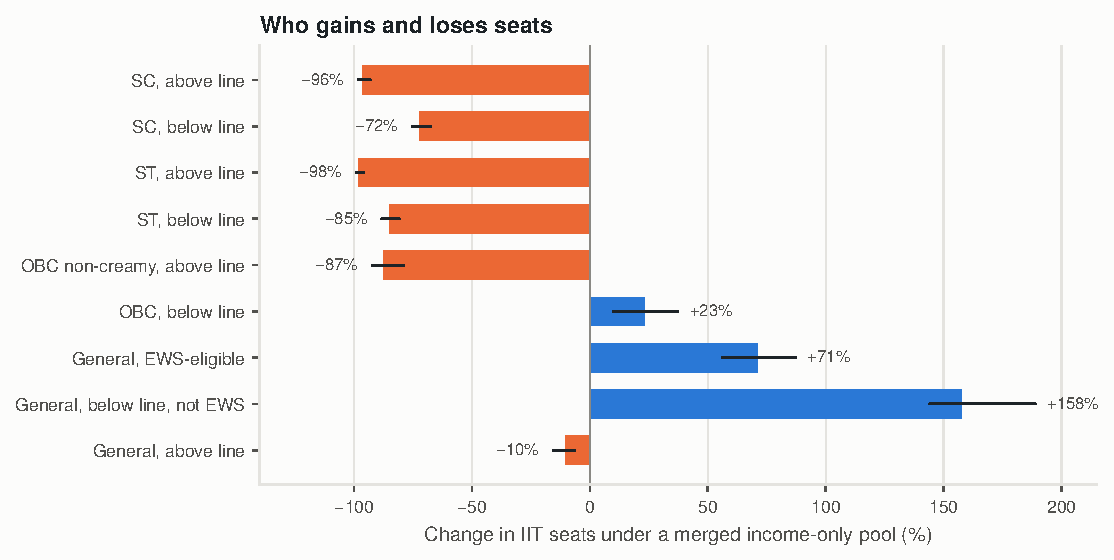
\includegraphics[width=0.92\linewidth]{../figures/fig10_allocation_seat_changes.pdf}
\caption{Change in IIT seats by group under a merged income-only pool (median, with 90\% intervals over the uncertainty about family incomes).}
\end{figure}

\section{Theory: why people would protest}

\subsection{Loss aversion and the politics of taking things away}
People weigh losses about twice as heavily as equal gains; Tversky and Kahneman estimate a loss-aversion coefficient of 2.25. Pierson's work on welfare retrenchment builds on this: cutting an existing benefit is harder than creating one, and governments that succeed use grandfathering, compensation for losers, and blame-sharing through broad coalitions.
\begin{plainwords}Taking away a quota feels worse than never having had one, and the people who lose are easier to organize than the people who gain.\end{plainwords}

\subsection{Symbolic threat and group identity}
For SC and ST communities, caste-based reservation is also a constitutional recognition of historical injustice. Removing caste as the basis therefore carries a symbolic threat independent of any individual's eligibility. The 2018 bandh, which followed a court ruling that removed no one's quota, is the clearest Indian evidence that symbolic threat alone can mobilize at national scale.
\begin{plainwords}Many people would protest because they read the change as erasing their community's recognition, whether or not they lose a seat.\end{plainwords}

\subsection{Threshold cascades}
Granovetter's threshold model treats each person as having a personal threshold: the share of others who must already be protesting before they join. Small differences in the distribution of thresholds or grievances can produce large differences in turnout.
\begin{plainwords}People join when enough of their neighbours already have. Lowering grievance a little can remove a large share of the protest, because fewer people join early and the chain reaction stops sooner.\end{plainwords}

\subsection{Organization}
Organizations, parties and networks supply the bandh calls and messaging that turn grievance into turnout. The 2018 bandh, however, was organized with little central leadership or party backing, through local groups and WhatsApp; the 2024 bandh had opposition-party backing and drew a mixed response. Party machinery is one amplifier among several, not a precondition.
\begin{plainwords}Protest needs organizing, but in 2018 local groups did it over WhatsApp, without party backing.\end{plainwords}

\subsection{Repression and backfire}
Studies of repression find that force sometimes deters and sometimes backfires. Rydzak finds that internet shutdowns in India are associated with more violent collective action, not less.
\begin{plainwords}Cutting the internet or sending in heavy policing may shrink the crowd on a given day, and it costs lives. Whether it also makes protest bigger depends on how people react to deaths.\end{plainwords}

\section{The model in simple terms}

\begin{figure}[H]
\centering
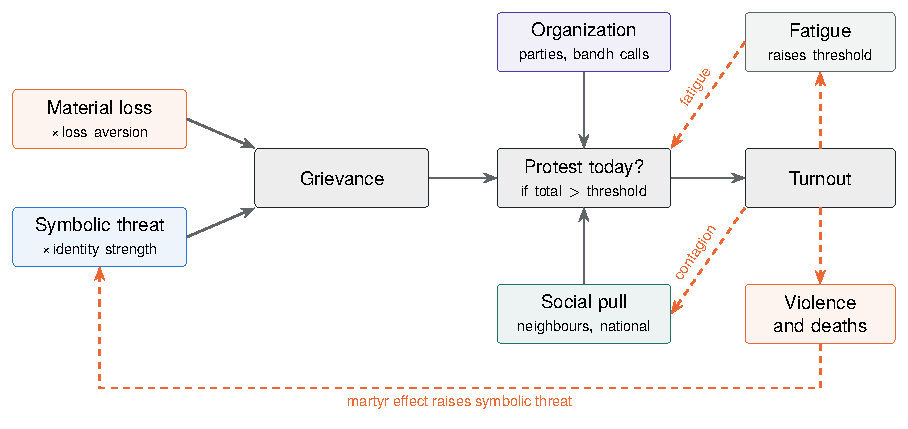
\includegraphics[width=0.95\linewidth]{../figures/fig00_mechanism.pdf}
\caption{What drives one person's decision each day. Dashed arrows are feedback loops: today's turnout shapes tomorrow's decisions.}
\end{figure}

\subsection{The synthetic India}
The model builds 120{,}000 agents, each standing for about 12{,}000 people, spread across India's 640 Census 2011 districts in proportion to population. Each district has its own SC and ST shares; OBC and General shares follow the state's figures from the National Family Health Survey. About one family in five sits above \rupee8 lakh. Agents live in neighbourhoods of about 100; most neighbourhoods are single-group, and the rest are mixed.

\subsection{How one day works}
For every agent, every day:
\begin{enumerate}
\item \textbf{Grievance} is the material loss (weighted 2.25 times if it is a loss), taken from the seat-allocation model, plus the symbolic threat multiplied by how strongly the agent identifies with its group.
\item \textbf{Social pull} rises with the share of the agent's neighbourhood that protested yesterday and with its group's national turnout. Both effects saturate.
\item \textbf{Organization} adds a push on bandh days. Organizations call a bandh when they expect a credible turnout.
\item The agent \textbf{protests} with a probability that rises smoothly as grievance plus pull plus push exceeds its personal threshold. Protesting raises the threshold a little (\textbf{fatigue}).
\item Deaths occur in proportion to turnout, most of them on bandh days, and raise symbolic threat for the groups on the street (the \textbf{martyr effect}).
\item The government may \textbf{concede} under pressure, which relieves grievance but can provoke a counter-mobilization by the General category.
\end{enumerate}

\subsection{Checking the model against real protests}
Protest turnout in India is rarely counted, and the estimates that exist differ by a factor of a hundred (for 2018, from ``thousands'' to ``hundreds of thousands''). Instead of a headcount, the model is checked against how many protest events the news reported, from the GDELT database, for four episodes: the SC/ST Bharat Bandhs of April 2018 and August 2024, the upper-caste bandh of September 2018, and the EWS amendment of January 2019, which drew little protest. Parameter sets that cannot reproduce all four are discarded; \CalibKept{} survive after \CalibWaves{} rounds of \CalibWaveSize{} sets each. The news counts pin down the relative size of past shocks, but they say little about how people behave: the surviving sets cover most of the range tried for every behavioural parameter.

Results of the check:
\begin{itemize}
\item The event data tell us how big the episodes were \emph{relative to each other} much better than how big they were. The surviving sets imply that \CalibTurnoutTwentyEighteenInterval{} lakh people joined the 2018 bandh.
\item When one episode was hidden from the model and predicted from the others, the predictions of deaths and of which states protest were weak. The model is a tool for comparing policy designs, not a forecast.
\end{itemize}

\section{Results at a glance}

\begin{figure}[H]
\centering
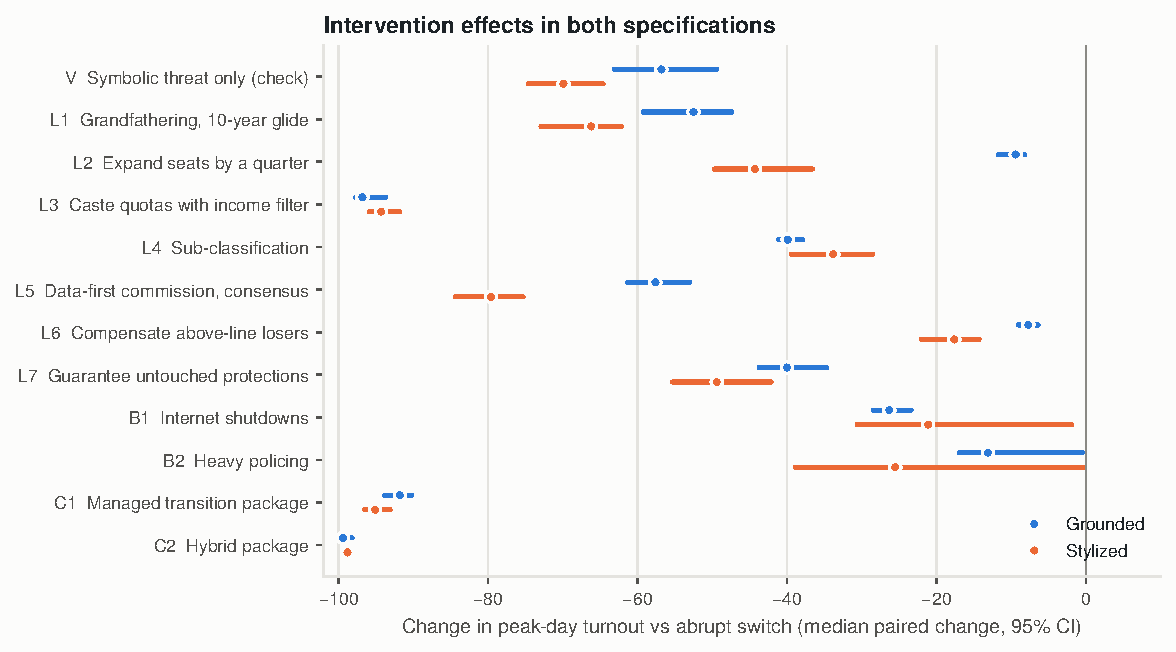
\includegraphics[width=\linewidth]{../figures/fig12_paired_effects.pdf}
\caption{Change in peak-day turnout for each option compared with the abrupt switch in the same simulated world. Dots are medians, lines 95\% intervals, for the data-grounded model and the original stylized model.}
\end{figure}

\begin{table}[H]
\centering\small
\caption{Grounded model, \RunCountGrounded{} paired runs per scenario. Peak in lakh; change is the median paired change with 95\% interval; ever protested in crore.}
\begin{tabularx}{\linewidth}{@{}lLrrrrrr@{}}
\toprule
 & Scenario & Peak & 10th--90th & Change & 95\% CI & Ever & Deaths\\
\midrule
\tablerows{generated/scenario_table_grounded_central.tex}
\bottomrule
\end{tabularx}
\end{table}

\begin{table}[H]
\centering\small
\caption{Stylized model, central regime, \RunCountCentral{} paired runs per scenario.}
\begin{tabularx}{\linewidth}{@{}lLrrrrrr@{}}
\toprule
 & Scenario & Peak & 10th--90th & Change & 95\% CI & Ever & Deaths\\
\midrule
\tablerows{generated/scenario_table_central.tex}
\bottomrule
\end{tabularx}
\end{table}

\paragraph{About the headcounts} The grounded model's baseline peak of \PeakGroundedBaseline{} rests on two things the data cannot settle: how strongly the reform would threaten caste recognition compared with the 2018 ruling, and how much material grievance weighs. Across the plausible range the peak runs from \AssumptionPeakLow{} to \AssumptionPeakHigh. The headcounts are illustrations; the changes between designs are the result.

\section{Where the anger comes from, and who protests}

\begin{figure}[H]
\centering
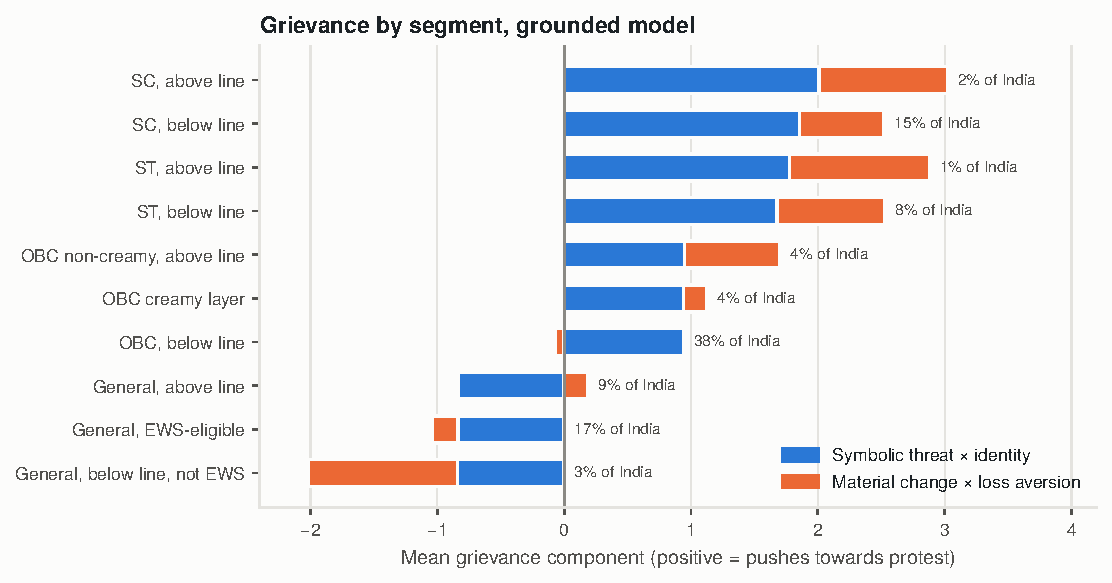
\includegraphics[width=0.9\linewidth]{../figures/fig16_grievance_composition_grounded.pdf}
\caption{Average grievance by group in the grounded model, split into symbolic threat and material change.}
\end{figure}

\begin{itemize}
\item \textbf{Symbolic and material grievance.} Symbolic threat is \SymbolicShareOfGrievance{} of all the grievance that pushes people towards protest. Removing it cuts the peak by \GChanNoSymbolic; removing the material losses cuts it by \GChanNoMaterial. For below-line SC and ST families, the seat losses add between a third and a half to their grievance.
\item \textbf{Who protests.} SC communities make up \GroupShareSC{} of protester-days and ST communities \GroupShareST.
\item \textbf{Where.} \TopStates. This is where the SC and ST population lives, not a prediction of where organizers will succeed: in 2018, Punjab, where the bandh call began, reported far more protest than its population share.
\end{itemize}

\begin{figure}[H]
\centering
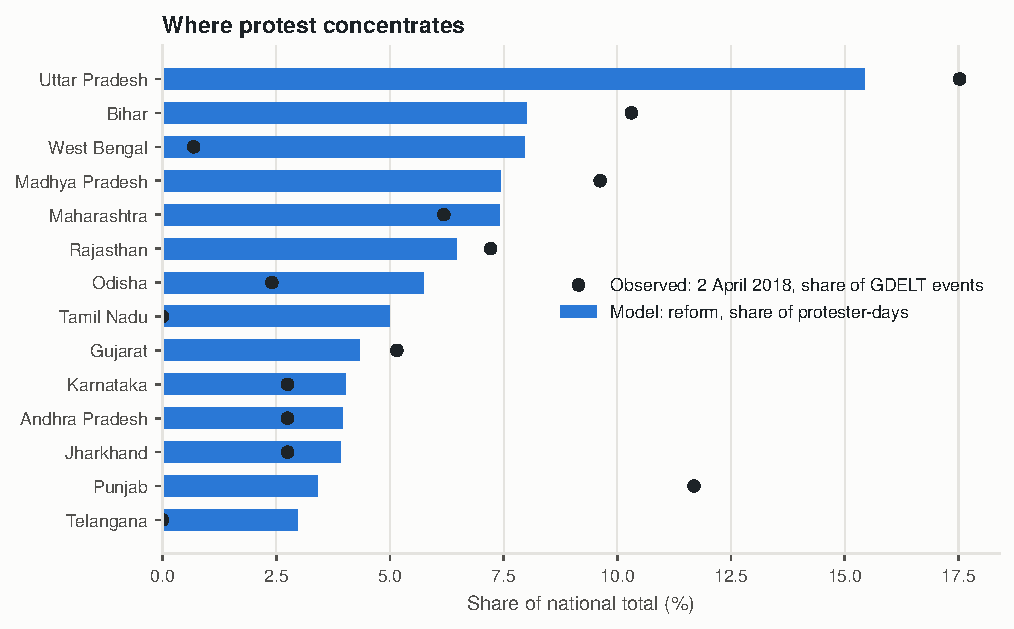
\includegraphics[width=0.9\linewidth]{../figures/fig17_state_distribution.pdf}
\caption{Share of protest by state in the grounded model, and the share of reported protest events by state on 2 April 2018.}
\end{figure}

\subsection{Patterns from past protests}
Five patterns from past episodes, and whether the model shows them:
\begin{enumerate}
\item A threat to recognition alone can bring out a national bandh: \textbf{yes}.
\item Protest concentrates on bandh days: \textbf{mostly} (bandh days are about \FactBandhToOrdinary{} times ordinary days).
\item Party backing is not what makes a bandh large: \textbf{yes} (raising party backing from the 2018 to the 2024 level changes the peak by a factor of only \FactBackingPeakRatio).
\item A group splits when a reform creates winners inside it: \textbf{yes} (sub-classification changes the poorest sub-castes' participation by \FactDeprivedChange).
\item Some bandhs turn deadly and governments concede: \textbf{partly}. Deaths and concessions happen in the model, but it cannot tell which bandhs will turn violent.
\end{enumerate}

\section{Scenario by scenario}

Each scenario follows the same layout: what the policy is, the theory behind it, a plain-language summary, how it enters the model, the outcome, and why. Changes compare peak-day turnout with the abrupt switch in the same simulated world.

\subsection{Base: the abrupt \rupee8 lakh income-only switch}
\subsubsection{What it is}
Parliament replaces SC, ST, OBC and EWS quotas with a single income test at \rupee8 lakh, effective immediately, with no consultation or transition.
\begin{plainwords}This is the reference point: the reform done in the most provocative way.\end{plainwords}
\subsubsection{Outcome}
\outcomeline{\PeakGroundedBaseline}{\PeakRangeGroundedBaseline}{--}{\CumulativeGroundedBaseline}{\DeathsGroundedBaseline}{\PeakCentralBaseline{} peak, \CumulativeCentralBaseline{} ever protest, \DeathsCentralBaseline{} deaths.}
\subsubsection{Why}
SC communities carry most of the turnout: they combine the highest symbolic threat, the strongest organizations and, according to the allocation model, the largest seat losses. In the grounded model the government concedes in \GroundedConcededShare{} of runs, after a median of \GroundedConcessionDay{} days.

\subsection{V: symbolic threat only (a check)}
\subsubsection{What it is}
All material loss is removed, so only the symbolic threat remains, much like the 2018 ruling.
\subsubsection{Outcome}
\outcomeline{\PeakGroundedSymbolicOnlyValidation}{\PeakRangeGroundedSymbolicOnlyValidation}{\PeakChangeGroundedSymbolicOnlyValidation}{\CumulativeGroundedSymbolicOnlyValidation}{\DeathsGroundedSymbolicOnlyValidation}{\PeakCentralSymbolicOnlyValidation{} (\PeakChangeCentralSymbolicOnlyValidation).}
\subsubsection{Why}
Symbolic threat alone still produces a large protest. Material loss matters more in the grounded model than in the stylized one, because the allocation model shows that below-line SC and ST students lose most of their seats, not a small share.

\subsection{L1: grandfather current cohorts, with a 10-year glide}
\subsubsection{What it is}
Students and job applicants already in the pipeline keep their current category rights. The income test is phased in over ten years.
\begin{plainwords}Nobody who is counting on a quota today loses it, and the change arrives slowly enough to plan around.\end{plainwords}
\subsubsection{How it is modelled}
Every material loss is cut to 30\% of its value; symbolic threat falls by 5\%.
\subsubsection{Outcome}
\outcomeline{\PeakGroundedGrandfathering}{\PeakRangeGroundedGrandfathering}{\PeakChangeGroundedGrandfathering}{\CumulativeGroundedGrandfathering}{\DeathsGroundedGrandfathering}{\PeakCentralGrandfathering{} (\PeakChangeCentralGrandfathering).}
\subsubsection{Why}
Grandfathering removes most of the material grievance, and in the grounded model material grievance is large. It does nothing about recognition.

\subsection{L2: expand seats}
\subsubsection{What it is}
Capacity grows by a quarter, the scale used to introduce EWS in 2019, and the merged pool fills the larger intake.
\begin{plainwords}Adding seats might mean that nobody loses theirs.\end{plainwords}
\subsubsection{How it is modelled}
The allocation model is rerun with 25\% more seats.
\subsubsection{Outcome}
\outcomeline{\PeakGroundedSeatExpansion}{\PeakRangeGroundedSeatExpansion}{\PeakChangeGroundedSeatExpansion}{\CumulativeGroundedSeatExpansion}{\DeathsGroundedSeatExpansion}{\PeakCentralSeatExpansion{} (\PeakChangeCentralSeatExpansion).}
\subsubsection{Why}
The EWS precedent does not transfer. EWS added a new category without merging any; here, even with a quarter more seats, the merged pool still ranks SC and ST candidates against General candidates, and below-line SC students still lose \AllocExpandedSCBelow{} of their seats. The stylized model assumed that expansion removes the loss, which is why it looked better there.

\subsection{L3: keep caste quotas, add an income filter inside them}
\subsubsection{What it is}
SC, ST and OBC quotas stay, but within each only families below the income line are eligible. In effect this extends the OBC creamy layer to SC and ST. Brazil's 2012 Quota Law combines criteria in a similar way.
\begin{plainwords}Keep the caste categories, but stop the richest families inside them from using the quota.\end{plainwords}
\subsubsection{How it is modelled}
For SC and ST, symbolic threat falls to the share implied by the 2024 bandh, which protested a creamy layer inside SC and ST quotas: a median of \LThreeRetainedMedian{} of the reform's threat, varying from run to run with the calibration. For OBC it falls to 40\%. The allocation model is rerun with SC and ST quotas closed to above-line families: their seats go to below-line SC and ST students, who gain (\AllocFilterSCBelow{} for SC, \AllocFilterSTBelow{} for ST).
\subsubsection{Outcome}
\outcomeline{\PeakGroundedHybridCasteSubquotas}{\PeakRangeGroundedHybridCasteSubquotas}{\PeakChangeGroundedHybridCasteSubquotas}{\CumulativeGroundedHybridCasteSubquotas}{\DeathsGroundedHybridCasteSubquotas}{\PeakCentralHybridCasteSubquotas{} (\PeakChangeCentralHybridCasteSubquotas).}
\subsubsection{Why}
It removes most of both drivers at once: the symbolic threat, and the seat losses of the below-line majority, which become gains. It is the strongest single option in most checks. Its symbolic relief comes from the 2024 bandh, so it is smaller and more uncertain than an assumed value would be. This design also keeps caste as a criterion, so it is an alternative to the reform rather than a version of it.

\subsection{L4: sub-classify to favour the most-deprived}
\subsubsection{What it is}
Within SC and ST, a larger share of benefits goes to the most-deprived sub-castes, as permitted by the Supreme Court in 2024.
\begin{plainwords}Give the poorest sub-castes a better deal, and many of them will not join the protest.\end{plainwords}
\subsubsection{How it is modelled}
The most-deprived tier's material loss falls by half a unit, and its symbolic threat falls from 0.8 to 0.3 times its group's. The better-off tier's symbolic threat rises by a fifth: in 2024, better-off SC groups protested sub-classification.
\subsubsection{Outcome}
\outcomeline{\PeakGroundedSubClassification}{\PeakRangeGroundedSubClassification}{\PeakChangeGroundedSubClassification}{\CumulativeGroundedSubClassification}{\DeathsGroundedSubClassification}{\PeakCentralSubClassification{} (\PeakChangeCentralSubClassification).}
\subsubsection{Why}
Participation in the most-deprived tier changes by \FactDeprivedChange, but the better-off tier reacts (\FactBetterOffChange), so the peak barely moves.

\subsection{L5: data-first commission with cross-party consensus}
\subsubsection{What it is}
The reform goes through a statutory commission that works from the caste census data before any legislation, with opposition parties represented.
\begin{plainwords}If every major party signs off, and the design is built on data everyone has seen, the reform reads less as an attack.\end{plainwords}
\subsubsection{How it is modelled}
The opposition-party amplifier falls from 1.5 to 1.0; symbolic threat falls by 20\%.
\subsubsection{Outcome}
\outcomeline{\PeakGroundedConsensusCommission}{\PeakRangeGroundedConsensusCommission}{\PeakChangeGroundedConsensusCommission}{\CumulativeGroundedConsensusCommission}{\DeathsGroundedConsensusCommission}{\PeakCentralConsensusCommission{} (\PeakChangeCentralConsensusCommission).}
\subsubsection{Why}
Most of the effect comes from the assumed cut in symbolic threat, not from withdrawing party machinery; in 2018 protest was large without it. Whether this option beats grandfathering depends on how much a commission would change what the reform means to people, which the model cannot tell.

\subsection{L6: compensate the families who lose eligibility}
\subsubsection{What it is}
Families that lose eligibility receive scholarships, hostel places and transitional grants.
\begin{plainwords}Pay the people who lose the quota.\end{plainwords}
\subsubsection{How it is modelled}
The losses of above-line SC, ST and non-creamy OBC families are halved.
\subsubsection{Outcome}
\outcomeline{\PeakGroundedCompensation}{\PeakRangeGroundedCompensation}{\PeakChangeGroundedCompensation}{\CumulativeGroundedCompensation}{\DeathsGroundedCompensation}{\PeakCentralCompensation{} (\PeakChangeCentralCompensation).}
\subsubsection{Why}
It reaches a small minority, not the below-line majority whose seats the merged pool takes, and money does nothing about symbolic threat.

\subsection{L7: guarantee untouched protections}
\subsubsection{What it is}
The reform is written with explicit guarantees about what stays untouched: SC/ST reserved seats in legislatures, the Atrocities Act, and a scheduled review clause.
\begin{plainwords}Say clearly, in law, what is not changing.\end{plainwords}
\subsubsection{How it is modelled}
Symbolic threat falls by 15\%.
\subsubsection{Outcome}
\outcomeline{\PeakGroundedCredibleGuarantees}{\PeakRangeGroundedCredibleGuarantees}{\PeakChangeGroundedCredibleGuarantees}{\CumulativeGroundedCredibleGuarantees}{\DeathsGroundedCredibleGuarantees}{\PeakCentralCredibleGuarantees{} (\PeakChangeCentralCredibleGuarantees).}
\subsubsection{Why}
A 15\% cut in symbolic threat produces a much larger cut in turnout, because the cascade multiplies any reduction.

\subsection{B1: internet shutdowns (tested for backfire)}
\subsubsection{What it is}
Mobile internet is suspended in areas with protests.
\subsubsection{How it is modelled}
Neighbourhood and national influence fall by 40\% and bandh mobilization by 20\%, while violent deaths rise 2.5 times.
\subsubsection{Outcome}
\outcomeline{\PeakGroundedInternetShutdown}{\PeakRangeGroundedInternetShutdown}{\PeakChangeGroundedInternetShutdown}{\CumulativeGroundedInternetShutdown{} (\CumulativeChangeGroundedInternetShutdown)}{\DeathsGroundedInternetShutdown{} (×\DeathRatioGroundedInternetShutdown)}{\PeakCentralInternetShutdown{} (\PeakChangeCentralInternetShutdown), deaths ×\DeathRatioCentralInternetShutdown.}
\subsubsection{Why}
Weaker coordination trims the peak. The rise in deaths is mostly the assumption itself: shutdowns are modelled as making protest more violent, following Rydzak's evidence.

\subsection{B2: heavy policing and mass arrests (tested for backfire)}
\subsubsection{What it is}
Large deployments, preventive detentions and forceful dispersal on bandh days.
\subsubsection{How it is modelled}
Turning out on bandh days costs more; deaths attributed to the police rise so that total deaths triple; each death raises symbolic threat half as much again.
\subsubsection{Outcome}
\outcomeline{\PeakGroundedHeavyPolicing}{\PeakRangeGroundedHeavyPolicing}{\PeakChangeGroundedHeavyPolicing}{\CumulativeGroundedHeavyPolicing{} (\CumulativeChangeGroundedHeavyPolicing)}{\DeathsGroundedHeavyPolicing{} (×\DeathRatioGroundedHeavyPolicing)}{\PeakCentralHeavyPolicing{} (\PeakChangeCentralHeavyPolicing), \CumulativeChangeCentralHeavyPolicing{} ever protest, deaths ×\DeathRatioCentralHeavyPolicing.}
\subsubsection{Why}
Policing lowers the peak a little and costs many lives. In the stylized model it also makes more people protest in total, because martyrs keep protest going between bandhs. In the grounded model it does not, because the government concedes within days. Whether force backfires on turnout depends on how people react to deaths, which none of the episodes can tell us. The rise in deaths holds in every version of the model, but it follows from the assumption that policing makes protest deadlier.

\subsection{C1: the managed-transition package}
\subsubsection{What it is}
Keep the income-only end state, but get there with seat expansion (L2), grandfathering (L1), a consensus commission (L5), compensation (L6) and guarantees (L7).
\subsubsection{Outcome}
\outcomeline{\PeakGroundedManagedTransition}{\PeakRangeGroundedManagedTransition}{\PeakChangeGroundedManagedTransition}{\CumulativeGroundedManagedTransition}{\DeathsGroundedManagedTransition}{\PeakCentralManagedTransition{} (\PeakChangeCentralManagedTransition).}
\subsubsection{Why}
Each component pushes people further below their thresholds, and because turnout responds non-linearly the combination does better than any single part.

\subsection{C2: the hybrid-design package}
\subsubsection{What it is}
L3 with sub-classification (L4), grandfathering (L1), the commission (L5), compensation (L6) and guarantees (L7).
\subsubsection{Outcome}
\outcomeline{\PeakGroundedHybridPackage}{\PeakRangeGroundedHybridPackage}{\PeakChangeGroundedHybridPackage}{\CumulativeGroundedHybridPackage}{\DeathsGroundedHybridPackage}{\PeakCentralHybridPackage{} (\PeakChangeCentralHybridPackage).}

\section{Can the reform survive?}
In the model the government concedes when protest is large, and it concedes against an abrupt switch in \ConcessionReferenceBaselineShare{} of runs, after a median of \ConcessionReferenceBaselineDay{} days. This rule is an assumption; no past episode fits anything after the first bandh day. With the strongest single option (L3) the government still concedes in \ConcessionReferenceShareLThree{} of runs; with the managed transition in \ConcessionReferenceShareCOne; with the hybrid package in \ConcessionReferenceShareCTwo. If governments concede more slowly, the shares fall to \ConcessionSlowShareLThree, \ConcessionSlowShareCOne{} and \ConcessionSlowShareCTwo.
\begin{plainwords}In the model, an income-only reform only lasts if it comes as a phased, negotiated package, and even then only if the government is slow to concede.\end{plainwords}

\section{How sure are these results?}
\label{sec:robustness}
\begin{itemize}
\item \textbf{How strongly each policy works is uncertain.} When every policy's strength is drawn at random from a wide range, keeping caste quotas with an income filter still comes first with probability \MapGroundedStrongestLThree. The commission beats grandfathering with probability \MapGroundedLFiveBeatsLOne{}, so grandfathering is more often the stronger of the two.
\item \textbf{The model's structure is uncertain.} Across \GEnsembleVariants{} alternative structures of the data-grounded model (different threshold shapes, fixed bandh days, no or slow concession, different death models, assumed instead of estimated seat losses), L3 comes first in \GEnsembleLThreeStrongest.
\item \textbf{Every parameter moved at once.} A Morris screen across fifteen parameters finds L3 ahead of the commission in \MorrisGroundedLThreeBeatsLFive{} of design points in the grounded model.
\item \textbf{Implausibly large crowds.} In \PlausibleShareBaselineAboveFiveCrore{} of runs the abrupt switch puts more than 5 crore people on the street in a day. Setting those aside, L3 still comes first in \PlausibleLThreeFirstBelowFiveCrore{} of the rest.
\item \textbf{What the data cannot settle.} Across the reform's shock size and party backing, the baseline peak moves from \AssumptionPeakLow{} to \AssumptionPeakHigh{}, but L3 comes first in all \AssumptionCells{} combinations.
\end{itemize}

\section{What this means}
\begin{enumerate}
\item \textbf{A merged income pool is not neutral.} It moves most seats of below-line SC and ST students to below-line General students, and adding seats on the EWS model does not undo that.
\item \textbf{Design matters more than compensation.} A design that keeps caste as the qualifier while filtering by income does far better than paying the people who lose.
\item \textbf{Lowering the peak is not enough.} In the model no single option makes it unlikely that the government backs down; only packages do.
\item \textbf{If the income-only end state is the goal,} phasing and a process that changes what the reform means matter most, and they compound.
\item \textbf{Suppression costs lives.} It lowers the peak less than most design options; whether it also broadens protest is uncertain.
\end{enumerate}

\subsection{Limitations}
\begin{itemize}
\item How strongly a commission, a guarantee or an income filter reduces the sense of threat is a judgement, handled with wide ranges.
\item News-event data pin down the relative size of past protests, not their headcounts, and they barely constrain how people behave in the model. The reform's protest level is therefore uncertain by more than tenfold.
\item When and whether the government concedes is an assumption, not an estimate.
\item The relevance of the news events was judged by a language model from the article links and has not yet been checked by hand.
\item The seat model covers IIT admissions only, the most selective institutions, and applies their losses to every family. Government jobs and other institutions may differ; scaling the losses down to a quarter leaves the ranking at the top unchanged.
\item Jati-level differences, state politics, courts, elections and media are not modelled.
\item Out-of-sample predictions of deaths and of which states protest were weak.
\end{itemize}

\section{Reproducing this report}
\begin{verbatim}
pip install -r requirements.txt
python -m experiments.merged_pool_allocation --draws 300
python -m experiments.episode_calibration --wave-size 6000 --waves 3
python -m experiments.compare_interventions --specification grounded
python -m experiments.compare_interventions --regime central
python -m visualization.render_grounded_figures
python -m visualization.write_latex_result_macros
python -m visualization.write_grounded_macros
cd report && xelatex research_report.tex && xelatex research_report.tex
\end{verbatim}
The paper's Reproducibility section lists every command.

\section*{References}
\begin{small}
\begin{itemize}[leftmargin=12pt,label={}]
\item Granovetter, M. (1978). Threshold models of collective behavior. \emph{American Journal of Sociology}, 83(6), 1420--1443.
\item Hess, D., \& Martin, B. (2006). Repression, backfire, and the theory of transformative events. \emph{Mobilization}, 11(2), 249--267.
\item Kahneman, D., \& Tversky, A. (1979). Prospect theory: An analysis of decision under risk. \emph{Econometrica}, 47(2), 263--291.
\item Leetaru, K., \& Schrodt, P. A. (2013). GDELT: Global data on events, location, and tone, 1979--2012. International Studies Association Annual Convention.
\item McCarthy, J. D., \& Zald, M. N. (1977). Resource mobilization and social movements: A partial theory. \emph{American Journal of Sociology}, 82(6), 1212--1241.
\item Pierson, P. (1994). \emph{Dismantling the Welfare State? Reagan, Thatcher, and the Politics of Retrenchment}. Cambridge University Press.
\item Rydzak, J. (2019). Of blackouts and bandhs: The strategy and structure of disconnected protest in India. SSRN Working Paper 3330413.
\item Daniyal, S. (2018). The WhatsApp wires: How Dalits organised the Bharat Bandh without a central leadership. \emph{Scroll.in}, 7 April 2018.
\item Sönmez, T., \& Yenmez, M. B. (2022). Affirmative action in India via vertical, horizontal, and overlapping reservations. \emph{Econometrica}, 90(3), 1143--1176.
\item Tajfel, H., \& Turner, J. C. (1979). An integrative theory of intergroup conflict. In W. G. Austin \& S. Worchel (Eds.), \emph{The Social Psychology of Intergroup Relations}. Brooks/Cole.
\item Tversky, A., \& Kahneman, D. (1992). Advances in prospect theory: Cumulative representation of uncertainty. \emph{Journal of Risk and Uncertainty}, 5(4), 297--323.
\item Government of India, affidavit in \emph{Janhit Abhiyan v. Union of India} (2022) on 2.14 lakh additional seats for EWS, as reported by The Tribune.
\item Brazil, Law No.\ 12.711 of 29 August 2012 (Quota Law).
\item \emph{State of Punjab v. Davinder Singh} (2024), Supreme Court of India, on sub-classification of Scheduled Castes.
\end{itemize}
\end{small}

\end{document}
